\documentclass[11pt]{article}

\author{Math 106}
\date{Due Friday, Sept 29 by 11:59pm} 
\title{Homework 3}

\usepackage{graphicx,xypic}
\usepackage{amsthm}
\usepackage{amsmath,amssymb}
\usepackage{amsfonts}
\usepackage{xcolor}
\usepackage[margin=1in]{geometry}
\usepackage[shortlabels]{enumitem}
\newtheorem{problem}{Problem}
\renewcommand*{\proofname}{{\color{blue}Solution}}


\setlength{\parindent}{0pt}
\setlength{\parskip}{1.25ex}


\begin{document}

\maketitle

% You are required to put your name here:
{\bf\Large Name:} 


\vspace{.3in}
Topics covered: curvature, Frenet frame, fundamental theorem of space curves, rotation number

Instructions: 
\begin{itemize}
\item This assignment must be submitted on Gradescope by the due date. 
\item If you collaborate with other students (which is encouraged!), please mention this near the corresponding problems. 
\item If you are stuck, please ask for help (from me, a TA, a classmate). Use ed discussions!  
\item You may freely use any fact proved in class. In general, you should provide proof for facts used that were not proved in class. 
\item Please restrict your solution to each problem to a single page. Usually solutions can be even shorter than that. If your solution is very long, you should think more about how to express it concisely.
\end{itemize}
\pagebreak 



\begin{problem}
Determine the rotation number of the following curves. Please show some work.
\begin{center}
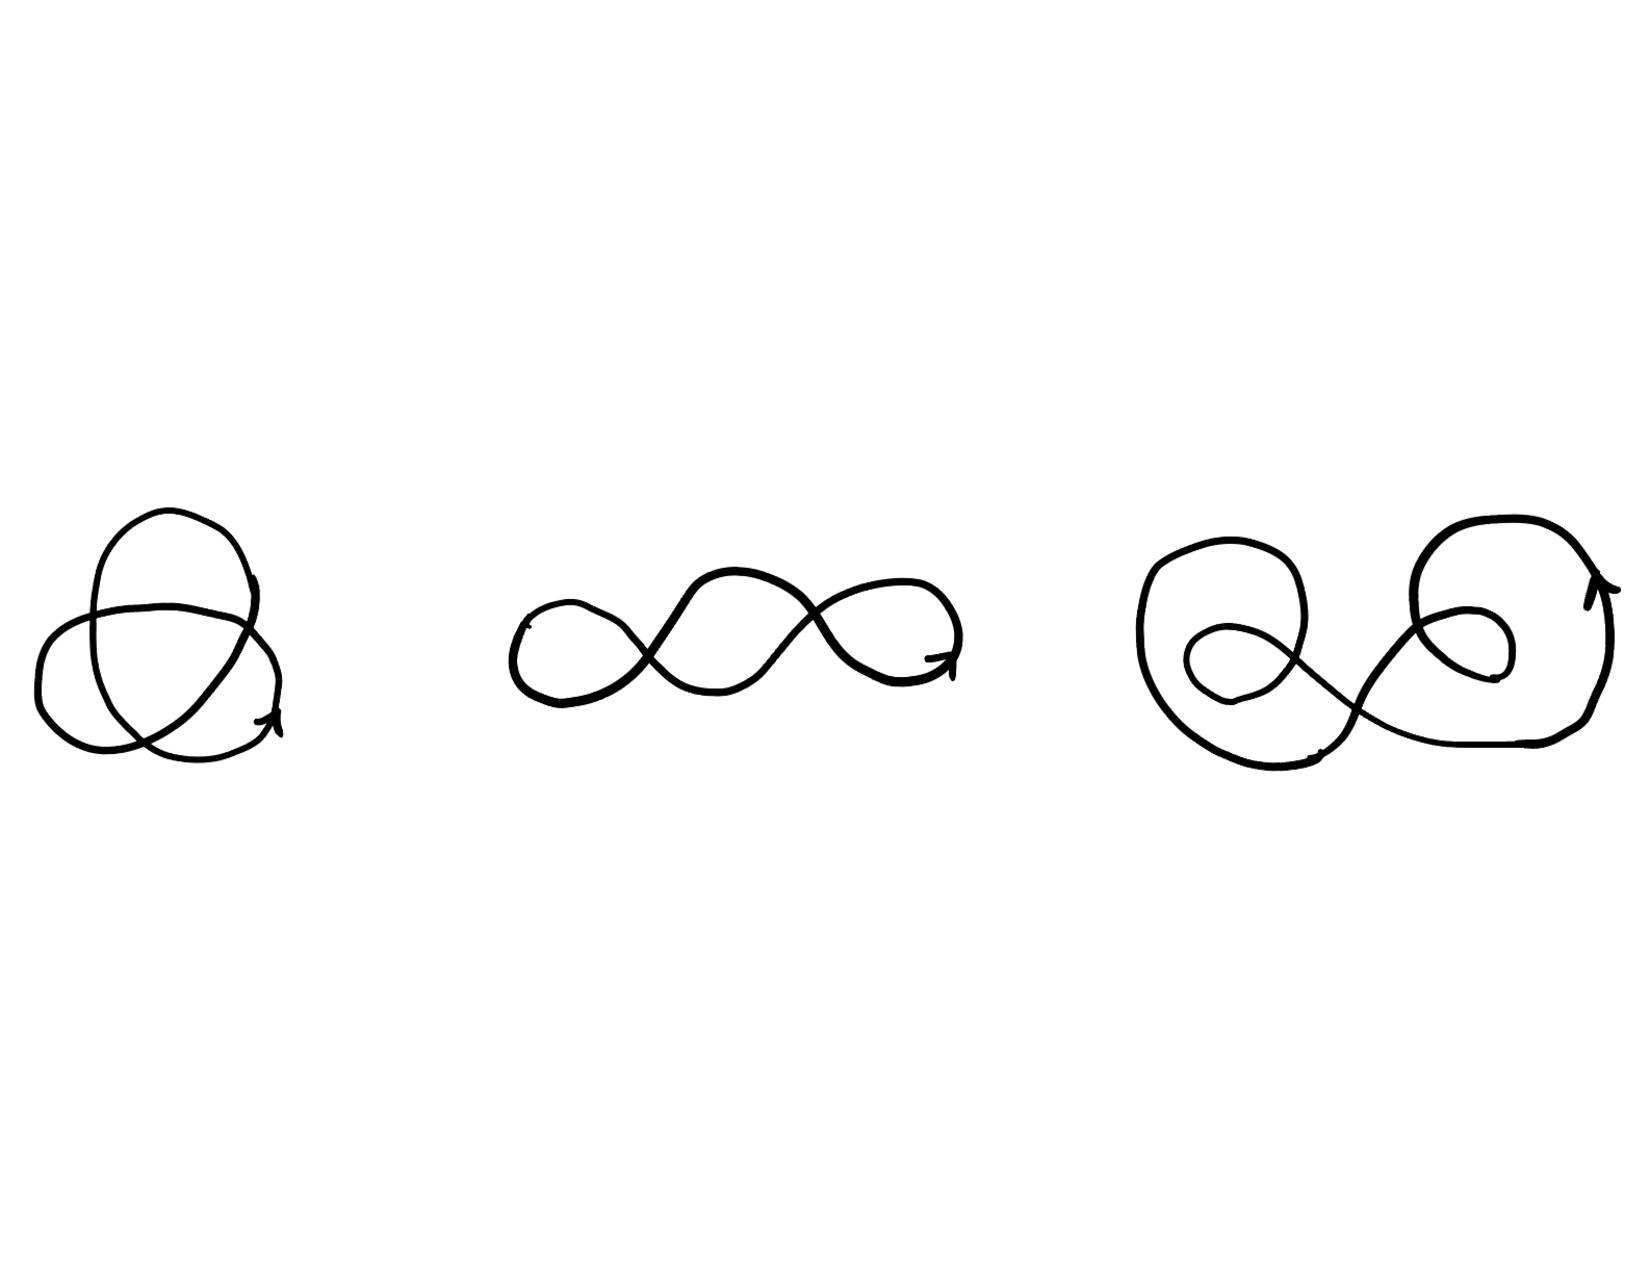
\includegraphics[scale=.5]{rot.pdf}
\end{center}
\end{problem}

\begin{proof}

\end{proof}



\pagebreak



\begin{problem}
Write down a linear system of differential equations in functions $f_1,\ldots,f_6$ that is  satisfied by $f_1=T\cdot N$, $f_2=T\cdot B$, $f_3=N\cdot B$, $f_4=T\cdot T$, $f_5=N\cdot N$, $f_6=B\cdot B$ when $T,N,B$ are a Frenet frame.\footnote{Hint: differentiate these dot product functions, and express the answer back in terms of these functions. The final answer should be a system of differential equations involving $f_1,\ldots,f_6$, not $T,N,B$.} Verify that the functions $f_1=f_2=f_3=0$ and $f_4=f_5=f_6=1$ is a solution to your system of differential equations.\footnote{Remark: recall this fact is used to prove the fundamental theorem of space curves.} 
\end{problem}

\begin{proof}

\end{proof}

\pagebreak

\begin{problem}
Let $F:V\to V$ be a linear operator on a finite-dimensional inner-product space. Prove the following are equivalent. 
\begin{enumerate} [(a)]
\item $F$ preserves the inner product. 
\item $F$ preserves lengths of vectors. 
\item $F$ preserves orthonormality (i.e.\ it sends an ONB to another ONB). 
\item $F$ preserves orthonormality of some orthonormal basis (i.e.\ there exists an ONB that is sent to an ONB under $F$).
\end{enumerate} 
A map satisfying these conditions is called a linear isometry or an orthogonal map.\footnote{Remark: for $\mathbb R^2$ with the standard inner product, the orthogonal maps are rotations and reflections.} 
\end{problem}

\begin{proof}

\end{proof}

\pagebreak

\begin{problem}
Show that the curvature and torsion of a curve are invariant under rigid motions. \footnote{Recall that (by our definition) a rigid motion is a composition of translations and orthogonal maps.} \footnote{Remark: this is the converse of the fundamental theorem of space curves.} \footnote{Hint: You'll probably need to show something about rigid motions and the cross product...}
\end{problem}

\begin{proof}

\end{proof}

\pagebreak

\begin{problem}For points $a,b,c$ in the plane, write $C(a,b,c)$ for the center of this circle that passes through $a,b,c$.\footnote{Fact: if $a,b,c$ do not lie on a line, then there is a unique circle passing through these points.} The osculating circle\footnote{Remark: the tangent line is the line that best approximates a curve at a point. Similarly, the osculating circle is the circle that best approximates a plane curve at a point.}  at $\alpha(t)$ is defined as the circle through $\alpha(t)$ with center 
\[C=\lim_{s\to0} C(\alpha(t-s),\alpha(t),\alpha(t+s)).\]
\begin{enumerate}[(i)]
\item Fix $\lambda>0$ and define $\beta(s)=(s,\lambda s^2)$. For $s\neq0$, compute the center of the circle that passes through $\beta(s),\beta(0)$, and $\beta(-s)$.  \footnote{Hint: First write the equation of a circle through a point $(a,b)$ with radius $r$. Then plug in $\beta(\pm s),\beta(0)$ and solve a system of equations to find $a,b,r$.}
\item Assume $\alpha$ satisfies $\alpha(0)=(0,0)$ and $\alpha'(0)=(1,0)$. Use the preceding part and the Taylor expansion of $\alpha(t)$ to show the radius of the osculating circle at $\alpha(0)$ is $1/\kappa$, where $\kappa=\kappa(0)$ is the curvature. \footnote{Hint: use specifically the degree-2 Taylor approximation.} \footnote{Remark: this problem gives a geometric interpretation for the curvature. }
\end{enumerate} 
\end{problem}

\begin{proof}

\end{proof}






\end{document}